\newsection{ALU}
\index{ALU}
\index{Arithmetic logic unit}
\index{Logic gate}
\label{alu}
The~abbreviation stands for~\textit{Arithmetic Logic Unit}.
It's an electronic circuit that performs arithmetic and~bitwise operations on~integer binary numbers.

\warning Do not confuse it with a~simple electronic device performing a~boolean operation over two bits (AND, OR, XOR etc.).
That's called \textit{Logic Gate}.
An~ALU consists of multiple logic gates.

\warning ALUs are parts of~CPUs, but not cores.
A~core is connected with an~ALU via an~execution port, sends inputs to it and processes returned results.
\newpage

\begin{figure}
    \centering
    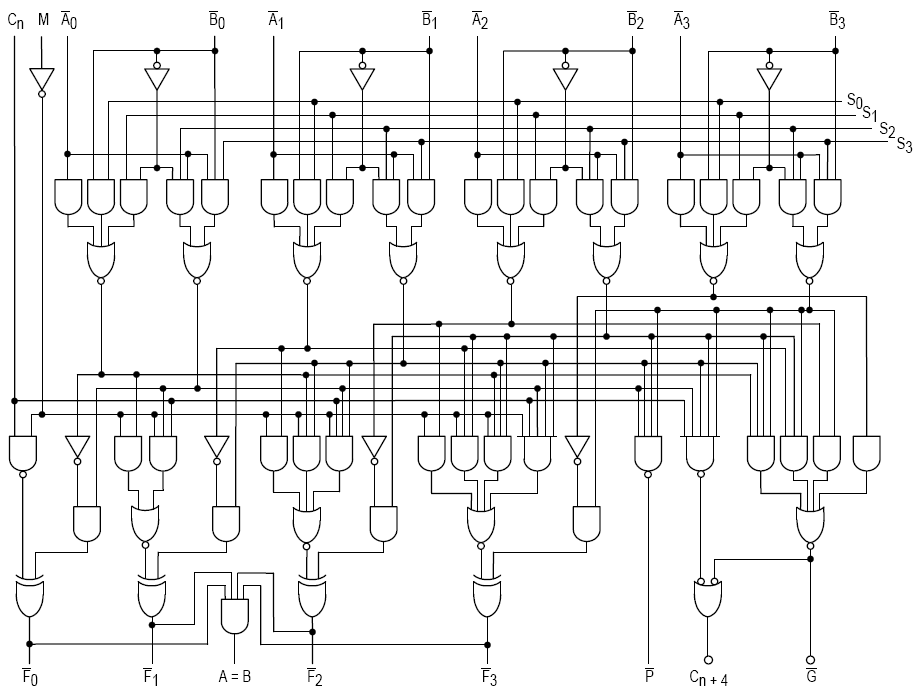
\includegraphics[width=\textwidth]{ALU.png}
    \captit{An example of a simple (no joke) four--bit ALU}
\end{figure}
